% Geometry, font
\documentclass[12pt, letter]{article}
\usepackage[margin=0.8in]{geometry}
\usepackage[T1]{fontenc}
\usepackage{fourier}
\usepackage{titling}
\setlength{\droptitle}{-5em} 
\usepackage[parfill]{parskip}
\usepackage{graphicx}
\usepackage{hyperref}

% Math stuff
\usepackage{amssymb}
\usepackage{bm}


\author{Zach Neveu}
\title{ Day 3: Intro to Comp. Complexity, P \& NP }

\begin{document}
\maketitle

\section{Review}%
\label{sec:review}
\begin{itemize}
	\item Huge difference between $O(n^k)$ and  $O(k^n)$ (Polynomial vs. Exponential)
	\item \underline{Intractable Problems} can only be solved (exactly) with an Exponential time algorithm
	\item Intractable $\ne$ Unsolvable!!
\end{itemize}

\section{New Stuff: Intractable Problems}%
\label{sec:new_stuff}
\subsection*{How to prove a problem is intractable?}
\begin{enumerate}
	\item If solution has size that is exponential, then any algorithm to find that solution can't be polynomial.
	\item If problem can't be solved by any algorithm at all (undecidable) - \href{https://en.wikipedia.org/wiki/Halting_problem}{Halting Problem}
	\item Certain niche problems with small output that are solvable but intractable
\end{enumerate}
\begin{figure}[h]
	\centering
	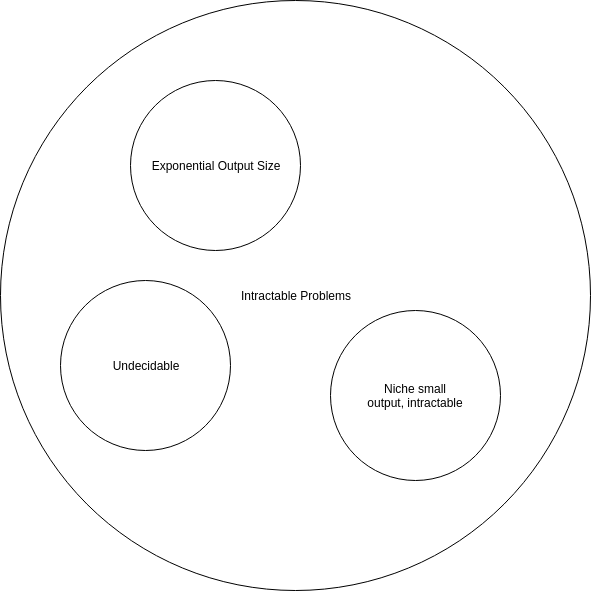
\includegraphics[width=0.5\textwidth]{imgs/intractable}
	\caption{Intractable Problem Categories}
	\label{fig:imgs-intractable}
\end{figure}

\section{NP-Completeness}%
\label{sec:np_completeness}

\subsection*{Properties}
\begin{itemize}
	\item No one has ever found a polynomial-time algorithm to solve
	\item If someone found one algorithm to solve a single NP complete problem in polynomial-time, it would solve all other NP-Complete problems too.
\end{itemize}

\begin{itemize}
	\item NP complete problems are either all tractable, or all intractable.
	\item All in same boat, we just don't know what boat.
	\item Tons of practical NP complete problems
	\item Seems unlikely that NP-Complete problems are tractable.
	\item It is widely believed that the NP-Complete problems are intractable.
\end{itemize}

\subsection*{What is NP-Complete?}
If you can't find an efficient algorithm what do you say?
\begin{itemize}
	\item "I can't find a solution" - get fired
	\item "A solution provably doesn't exist" - exceedingly unlikely
	\item "I can't solve it, but neither can anyone" - show that NP-Complete
\end{itemize}

\subsection*{Decision vs. Optimization Problems}
\begin{itemize}
	\item Computational Complexity initially developed for decision problems
	\item Must prove that it can be applied to optimization problems as well
	\item TSP-opt - Given weighted graph, find shortest Hamiltonian cycle - optimization problem
	\item TSP-dec - Given weighted graph, is there a Hamiltonian Cycle with weight $\le k$
	\item Knapsack-opt - Given objects w/ values and sizes and size bound, find subset to maximize values within size bound.
	\item Knapsack-dec - Given objects w/ values and sizes and size bound, is there a subset of the objects that are within the size bound and have a value $\ge k$.
	\item If optimization is tractable, then decision is tractable - just plug in answer from optimization
	\item If decision is tractable, then optimization is also tractable - just run binary search over $k$ values (adds log of constant)
	\item Decision and Optimization always have same complexity
\end{itemize}

\section{Complexity Classes}%
\label{sec:complexity_classes}
\subsection*{P}
\begin{itemize}
	\item The set of all decision problems that can be solved by a polynomial-time algorithm.
	\item HC Problem: Given a graph, is it Hamiltonian (does it contain at least one Hamiltonian cycle)?
\end{itemize}
\begin{figure}[h]
	\centering
	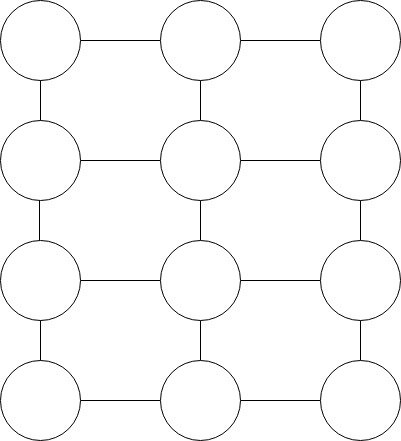
\includegraphics[width=0.4\textwidth]{imgs/hc}
	\caption{Does this graph have a Hamiltonian Cycle?}
	\label{fig:imgs-hc}
\end{figure}

\begin{itemize}
	\item A \underline{Verification Algorithm} takes some information and checks it to make sure it satisfies the problem requirements.
	\item Example: given a cycle, verify that it is in fact Hamiltonian
	\item A \textbf{Yes Instance} of a problem will have some certificate that a verification algorithm can verify
	\item a  \textbf{No Instance} will not contain a valid certificate to be verified
	\item Example: TSP-dec
	\begin{itemize}
		\item certificate: sequence of nodes in the found HC
		\item Verification algorithm: Check that each node appears once, edges are valid, and $\sum weights \le k$
	\end{itemize}
	\item Example: Matching - given graph and k, is there a matching of size k?
	\begin{itemize}
		\item Certificate: list of edges in found matching
		\item Verification algorithm: make sure no two edges have same end point, edges exist, and number of edges is k
	\end{itemize}
	\item Shortest Path - given graph, source and dest nodes, and k is there a path from start to end cheaper or equal to k?
	\begin{itemize}
		\item certificate: ordered nodes in the path found
		\item verification: check that edges exist, $\sum weight \le k$
	\end{itemize}
\end{itemize}

\subsection*{NP}


\end{document}
